\documentclass[11pt,a4paper]{article}

\usepackage[T1]{fontenc}
\usepackage[utf8]{inputenc}
\usepackage[english]{babel}
\usepackage[margin=2.5cm]{geometry}
\usepackage{amsmath}
\usepackage{amssymb}
\usepackage{graphicx}
\usepackage{xcolor}
\usepackage{listings}
\usepackage{float}
\usepackage{hyperref}

% --- metadata (agent: auto-fill practice id/title only) ---
\newcommand{\practiceid}{1}
\newcommand{\practicetitle}{Practice 1}
\newcommand{\reportauthors}{Arnau Torret \& Arnau Montull}
\newcommand{\reportdate}{\today}
\newcommand{\ph}[1]{\emph{[#1]}}

\hypersetup{
  colorlinks=true,
  linkcolor=blue,
  urlcolor=blue,
  citecolor=blue,
  pdftitle={\practicetitle},
  pdfauthor={\reportauthors}
}

\definecolor{codebg}{RGB}{247,247,247}
\definecolor{codeframe}{RGB}{200,200,200}
\definecolor{codekw}{RGB}{0,71,171}
\definecolor{codetype}{RGB}{11,110,79}
\definecolor{codeattr}{RGB}{125,60,152}
\definecolor{codestr}{RGB}{163,21,21}
\definecolor{codecmt}{RGB}{106,115,125}

% listings has no [free]Fortran dialect; define free-form Fortran 90 here.
\lstdefinelanguage{Fortran90}{
  sensitive=false,
  alsoletter={_},
  morekeywords=[1]{
    program,end,if,then,else,elseif,endif,do,while,enddo,
    call,return,contains,subroutine,function,module,use,only,
    select,case,default,exit,cycle,stop,continue,
    allocate,deallocate,open,close,read,write,print,
    include,implicit,none,interface,procedure,result,
    where,elsewhere,block,pure,elemental,recursive
  },
  morekeywords=[2]{
    integer,real,double,precision,complex,logical,character,
    type,class,kind
  },
  morekeywords=[3]{
    parameter,dimension,allocatable,intent,in,out,inout,
    optional,pointer,target,save,public,private,external,
    intrinsic,contiguous,value
  },
  morecomment=[l]!,
  morestring=[b]',
  morestring=[b]"
}

\lstdefinestyle{fortranstyle}{
  language=Fortran90,
  basicstyle=\ttfamily\footnotesize,
  backgroundcolor=\color{codebg},
  keywordstyle=[1]\color{codekw}\bfseries,
  keywordstyle=[2]\color{codetype}\bfseries,
  keywordstyle=[3]\color{codeattr},
  commentstyle=\color{codecmt}\itshape,
  stringstyle=\color{codestr},
  numbers=left,
  numberstyle=\tiny\color{gray},
  numbersep=8pt,
  frame=single,
  rulecolor=\color{codeframe},
  breaklines=true,
  showstringspaces=false,
  keepspaces=true,
  columns=fullflexible,
  tabsize=4,
  captionpos=b,
  xleftmargin=2em,
  framexleftmargin=1.5em
}
\lstdefinestyle{datastyle}{
  language={},
  basicstyle=\ttfamily\footnotesize,
  backgroundcolor=\color{codebg},
  numbers=left,
  numberstyle=\tiny\color{gray},
  numbersep=8pt,
  frame=single,
  rulecolor=\color{codeframe},
  breaklines=true,
  showstringspaces=false,
  keepspaces=true,
  columns=fullflexible,
  tabsize=4
}
\lstset{style=fortranstyle}

\begin{document}

\hypersetup{pageanchor=false}
\begin{titlepage}
\centering
\vspace*{1.5cm}

\includegraphics[width=5cm]{../../upc-logo.png}\\[1.2cm]

{\large\bfseries UNIVERSITAT POLITÈCNICA DE CATALUNYA}\\[0.45cm]
{\small Escola Tècnica Superior d'Enginyeria de Telecomunicacions de Barcelona (ETSETB)}

\vspace{3.2cm}

{\LARGE\bfseries \practicetitle}\\[1.1cm]
{\large Grau en Enginyeria Física}

\vfill
\begin{flushright}
\textbf{Authors:} \reportauthors\\[0.35cm]
\textbf{Subject:} SIMCOM\\[0.35cm]
\textbf{Date:} \reportdate
\end{flushright}
\end{titlepage}
\hypersetup{pageanchor=true}

% --- BEGIN EXERCISES ---

\section{Exercise 1}

\subsection{Question}
Write a full program that adds one integer with one real. Be sure to use correct style (program name, no implicit typing, correct declarations). Add the user to enter the two numbers. Print the result in an external file.

\subsection{Code}
\lstinputlisting[style=fortranstyle,label={lst:ex1}]{../ex1/ex1.f90}

\subsection{Results}
\begin{figure}[H]
  \centering
  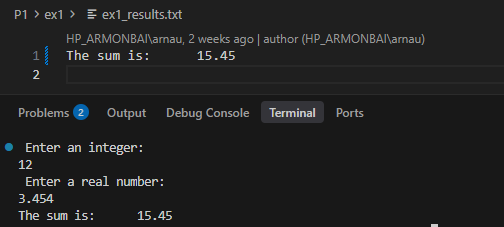
\includegraphics[width=0.9\linewidth]{../ex1/ex1_photo.png}
  \caption{Screenshot of exercise 1}
  \label{fig:ex1}
\end{figure}

\subsection{Discussion \& Notes}
As can be observed in the image, the program firstly ask the user for 1 integer and after the user insert it, the program asks for 1 real number. Finally, the program prints the result of the sum of the two numbers in an external file called \texttt{ex1\_results.txt}.

\newpage
\section{Exercise 2}

\subsection{Question}
{\sloppy
Use the Leibniz formula to compute $\pi$:
\begin{equation}
  \frac{\pi}{4} = \sum_{k=0}^{\infty} \frac{(-1)^k}{2k+1}
\end{equation}
Compute until your result agrees to at least five decimal digits within the correct value ($3.1415926535897932384626433\dots$). This series converges very slowly so this can take a lot of iterations\dots Display a graph showing the evolution with $k$, i.e.\ $\pi(k)$ as a function of $k$.
\par}

\subsection{Code}
\lstinputlisting[style=fortranstyle,label={lst:ex2}]{../ex2/ex2.f90}

\subsection{Results}
\begin{figure}[H]
  \centering
  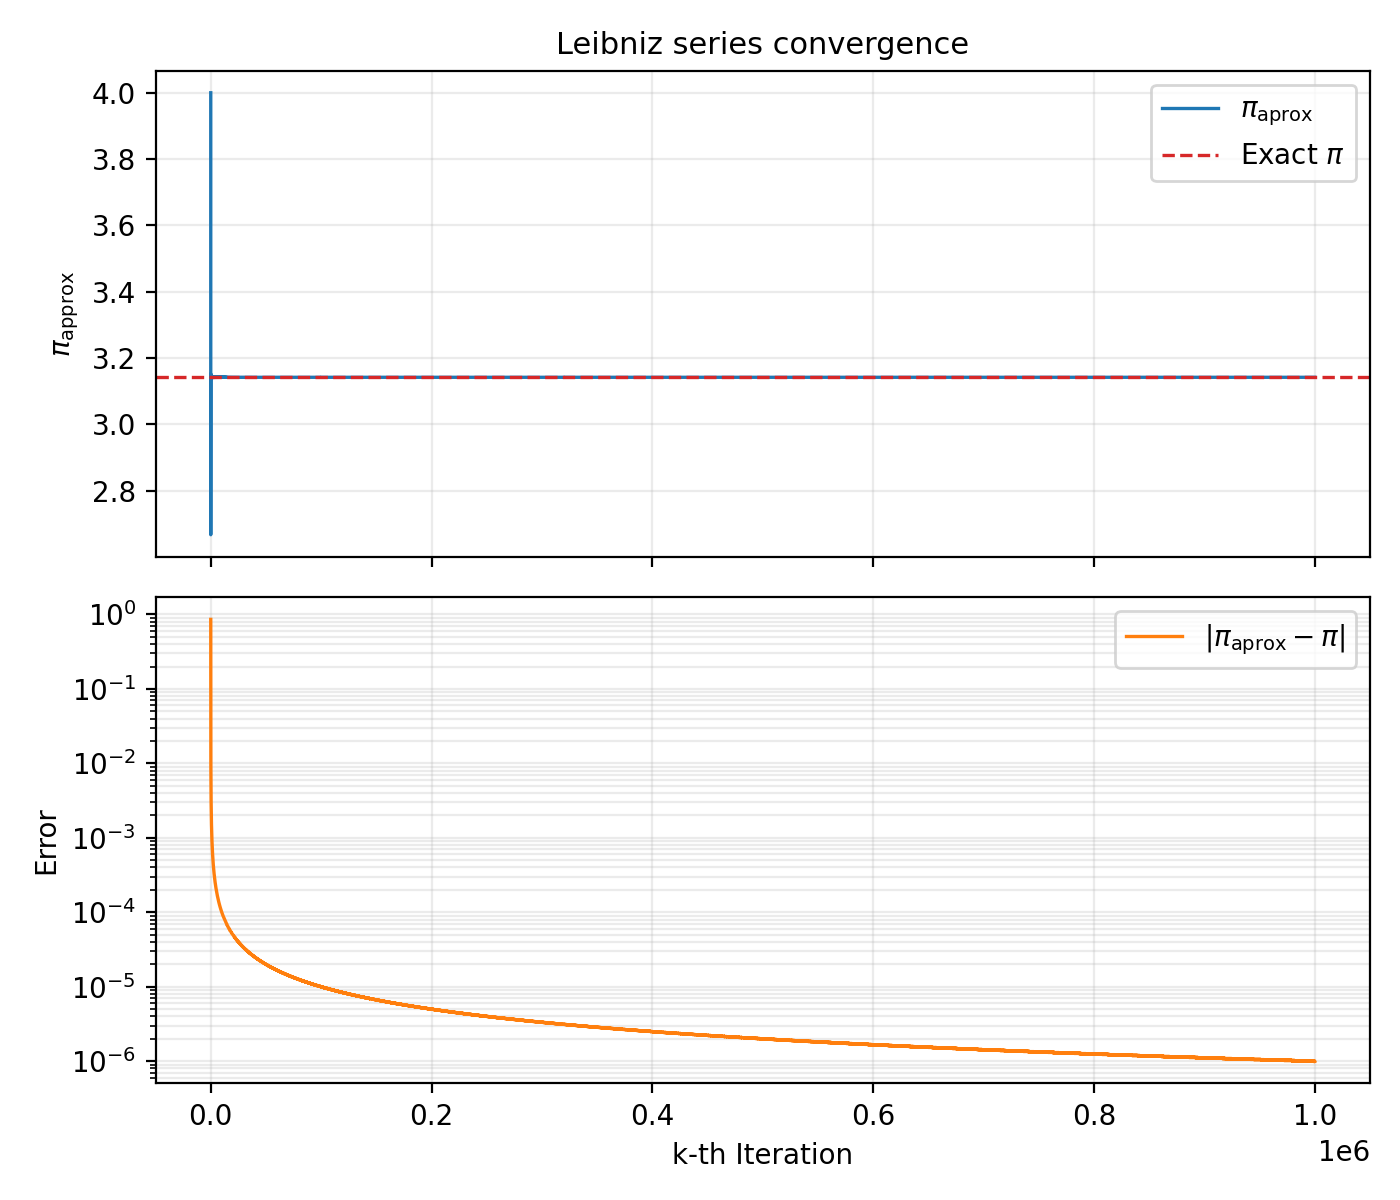
\includegraphics[width=0.75\linewidth]{../ex2/ex2_plot.png}
  \caption{Output of exercise 2}
  \label{fig:ex2}
\end{figure}

\subsection{Discussion \& Notes}
As we use the alternating Leibniz series to approximate $\pi$ until the first five decimal places converge, we require an error tolerance one order of magnitude smaller ($|\varepsilon| < 10^{-6}$) to guarantee this accuracy. Alternatively, we could have truncated both the reference value and our approximation to five decimal digits and checked for zero difference. However, because the partial sums oscillate around the true value, we could have satisfied that condition prematurely simply by chance. For this reason, to ensure consistency and robustness in our results, we enforced an error threshold strictly below $10^{-6}$.
\\ 
Therefore, to obtain $\pi$ with the desired accuracy, we need to compute the series until $K = 10^6$.

\newpage
\section{Exercise 3}

\subsection{Question}
Use subroutines and/or functions to write a code to compute the Fourier integral of a given time-dependent correlation function such as $C(t) = \langle A(0)\cdot A(t) \rangle$. For instance, in molecular water simulations, spectral lineshapes $I(\omega)$ are usually found from:
\begin{equation}
  I(\omega) \sim \frac{2Nq^2}{\pi\omega^2} S(\omega) \equiv \frac{2Nq^2}{\pi\omega^2} \int_0^{\infty} dt\,\langle\vec{v}_{H_i}(t)\cdot\vec{v}_{H_i}(0)\rangle \cos(\omega t)
\end{equation}
Use the same idea to obtain $S(\omega)$ for $C(t)$, given that it is read from a known file, say file named \texttt{corr.dat} (corresponds to an oxygen velocity autocorrelation), with the usual two-column format ($t$, $C(t)$). You will find the file at the ATENEA database. Note that the time step used in \texttt{corr.dat} is of $0.0005\text{ ps}$.

Find:
\begin{equation}
  S(\omega) = \int_0^{\infty} dt\, C(t)\cdot \cos(\omega t)
  \label{eq:fourier_cosine}
\end{equation}

\subsection{Code}
\lstinputlisting[style=fortranstyle,caption={Fortran implementation of composite Simpson's quadrature for the Fourier cosine transform.},label={lst:ex3}]{../ex3/ex3.f90}

\subsection{Results}
The input signal $C(t)$ and the resulting Fourier cosine transform spectrum $S(\omega)$ are illustrated in Figure~\ref{fig:ex3}.

\begin{figure}[H]
  \centering
  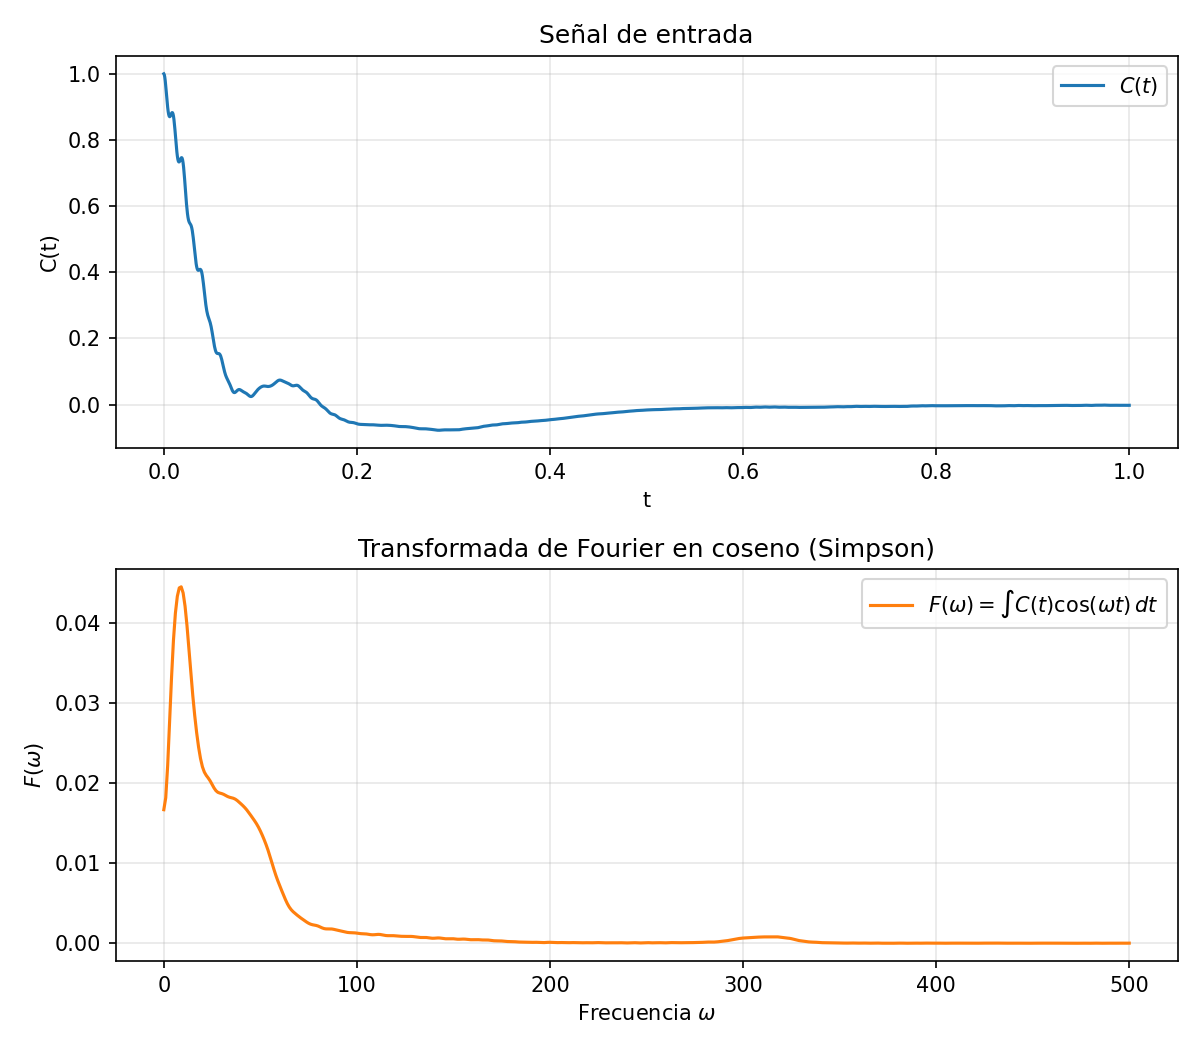
\includegraphics[width=0.9\linewidth]{../ex3/ex3_plot.png}
  \caption{Top: Input time-domain signal $C(t)$ over $t \in [0, 1]\text{ ps}$. Bottom: Fourier cosine transform $S(\omega) = \int C(t)\cos(\omega t)\,dt$ computed via composite Simpson's rule for $\omega \in [0, 500]\text{ ps}^{-1}$.}
  \label{fig:ex3}
\end{figure}

\subsection{Discussion \& Notes}
\begin{itemize}
  \item The numerical integration was carried out using the composite Simpson's 1/3 rule. The dataset contains $N = 2001$ points with a uniform time step of $\Delta t = 0.0005\text{ ps}$, which yields an even number of intervals ($N - 1 = 2000$), strictly satisfying the condition required for the standard Simpson's rule.

  \item We implemented the integration routine into a dedicated Fortran subroutine, \texttt{simpson(C, t, result)}. For each frequency value in the range $\omega \in [0, 500]\text{ ps}^{-1}$, the integrand $f(t) = C(t)\cos(\omega t)$ is evaluated and integrated over the full time domain.

  \item The computed spectrum $S(\omega)$ matches the reference curve from the presentation: a dominant low-frequency peak located around $\omega \approx 10\text{ ps}^{-1}$, followed by a gradual decay and a smaller secondary local maximum near $\omega \approx 315\text{ ps}^{-1}$.
\end{itemize}

\newpage
\section{Exercise 4}

\subsection{Question}
Compute integrals with the MC method, using random sampling.

\paragraph{Calculation of a surface:}
Idea: Use of the mean value theorem for integrals. The value of the integral is:
\begin{equation}
  \int_a^b dx\, f(x) = (b - a)\langle f \rangle, \quad \text{where} \quad \langle f \rangle_N = \frac{1}{N}\sum_{i=1}^N f(x_i)
\end{equation}
Evaluate the area enclosed between the curves $y = x^{-1}$ and $y = -x^{-1}$ within the range $x \in [-1, 1]$ and $y \in [-11, 11]$, represented in the figure. Note that the exact value is $A_{\text{exact}} = 13.5916$.

\paragraph{Procedure:}
\begin{enumerate}
  \item[A.] Generate $N$ points $(x_i, y_i)$ at random. $x_i$ belongs to a uniform distribution in the range $[-1, 1]$ and $y_i$ belongs to a uniform distribution in the range $[-11, 11]$. (\textit{Hint: You will need a good random number generator! Try \texttt{RANDOM\_SEED}, works in most of Fortran versions}).
  \item[B.] Calculate the number of points $N_{\text{hit}}$ inside the region of interest and estimate the area as follows:
  \begin{equation}
    A(N) = 2 \times 22 \times \frac{N_{\text{hit}}}{N}
  \end{equation}
  \item[C.] Run a number of different MC series (for instance, 3) with $N = \{10^2 - 10^7\}$. For each $N$, calculate the mean value of the area:
  \begin{equation}
    \langle A(N) \rangle = \frac{1}{M}\sum_{i=1}^M A_i(N)
  \end{equation}
  and the standard deviation $\sigma$ (variance defined as $\sigma^2$):
  \begin{equation}
    \langle \sigma(N) \rangle = \sqrt{\langle (A(N) - A_{\text{exact}})^2 \rangle}
  \end{equation}
  \item[D.] Finally plot $A(N)$ and $\sigma(N)$.
\end{enumerate}

\subsection{Code}
\lstinputlisting[style=fortranstyle,label={lst:ex4}]{../ex4/ex4.f90}

\subsection{Results}
\begin{figure}[H]
  \centering
  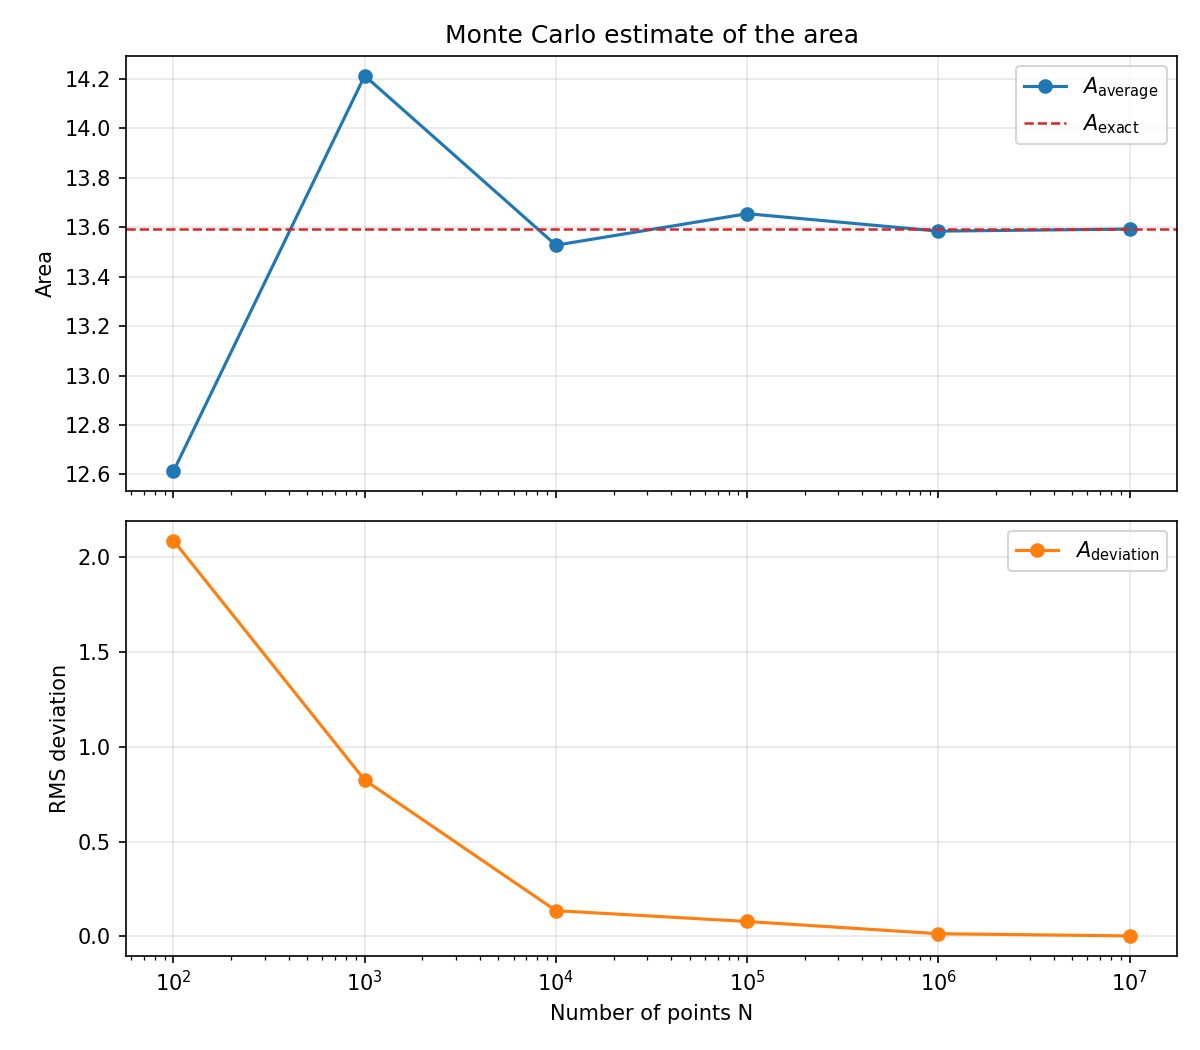
\includegraphics[width=0.75\linewidth]{../ex4/ex4_plot.png}
  \caption{Output of exercise 4}
  \label{fig:ex4}
\end{figure}

\subsection{Discussion \& Notes}
\begin{itemize}
  \item \textbf{Simulation setup and method:} 
  We tested sample sizes from $N = 100$ up to $10^7$, running each test $3$ times. In each run, we picked $N$ random points $(x, y)$ inside a rectangle of width $2$ and height $22$ (total area $= 44$). A point counts as a ``hit'' if it lands under the curve ($|y| \le |1/x|$). We then estimated the area using:
  \[
  \text{Area} = 44 \times \frac{\text{Hits}}{N}
  \]
  Finally, we averaged the $3$ runs and calculated how far the result was from the true value, $A_{\text{exact}} \approx 13.5916$.

  \item \textbf{Code details:} 
  To avoid dividing by zero when calculating $1/x$, the code checks \texttt{IF (x /= 0.0)} before testing a point; skipping this single line does not change the calculated area.
  
  \item \textbf{Sweet spot:}
  As $N$ increases, the estimated area converges toward the analytical value ($13.5916$), with the error decreasing as $1/\sqrt{N}$, as expected for Monte Carlo integration:
  \begin{itemize}
    \item At $N = 10^2$, the relative error is substantial ($\approx 15\%$).
    \item By $N = 10^4$, the error drops to approximately $1\%$.
    \item At $N = 10^6$, the error reaches $\approx 0.1\%$, providing high precision within seconds.
    \item At $N = 10^7$, the estimate ($13.592$) matches the true value to three decimal places ($< 0.02\%$ error).
  \end{itemize}
  Since no target accuracy was explicitly specified, $N = 10^6$ serves as the optimal trade-off: it achieves sub-percent accuracy ($\sim 0.1\%$) with minimal runtime, whereas scaling to $N = 10^7$ increases computation time by a factor of 10 for only a modest threefold gain in precision.\end{itemize}
\newpage
\newpage
\section{Exercise 5}

\subsection{Question}
Consider an harmonic oscillator of mass $m = 200\text{ g}$ and force constant $k = 2\text{ N/m}$. Integrate numerically the equation of motion and compare the results of positions and velocities with the exact analytical solution. Compute also the kinetic, potential and total energies.

\paragraph{Initial position and velocity:} $x_0 = 5\text{ cm}$, $v_0 = 0$.

\paragraph{Integration algorithms and timesteps:}
\begin{itemize}
  \item Euler: $\Delta t = 0.001\text{ s}$, $\Delta t = 0.01\text{ s}$, $\Delta t = 0.02\text{ s}$
  \item Euler predictor-corrector: $\Delta t = 0.02\text{ s}$
  \item Verlet: $\Delta t = 0.02\text{ s}$
\end{itemize}

\subsection{Code}
\lstinputlisting[style=fortranstyle,caption={Fortran implementation of explicit Euler, Euler Predictor-Corrector, and Velocity-Verlet algorithms.},label={lst:ex5}]{../ex5/ex5.f90}

\subsection{Results}
The equations of motion for the simple harmonic oscillator ($m = 0.200\text{ kg}$, $k = 2\text{ N/m}$, $x_0 = 0.05\text{ m}$, $v_0 = 0\text{ m/s}$) were integrated up to $t_{\max} = 10\text{ s}$ using the explicit Euler scheme ($\Delta t \in \{0.001, 0.01, 0.02\}\text{ s}$), the Euler Predictor-Corrector scheme ($\Delta t = 0.02\text{ s}$), and the Velocity-Verlet algorithm ($\Delta t = 0.02\text{ s}$).

Figure~\ref{fig:ex5_pos} displays the simulated trajectories $x(t)$ compared against the analytical solution $x(t) = x_0 \cos(\omega_0 t)$, highlighting the effect of the step size $\Delta t$ on Euler's method as well as the comparison across all three integrators at $\Delta t = 0.02\text{ s}$.

\begin{figure}[H]
  \centering
  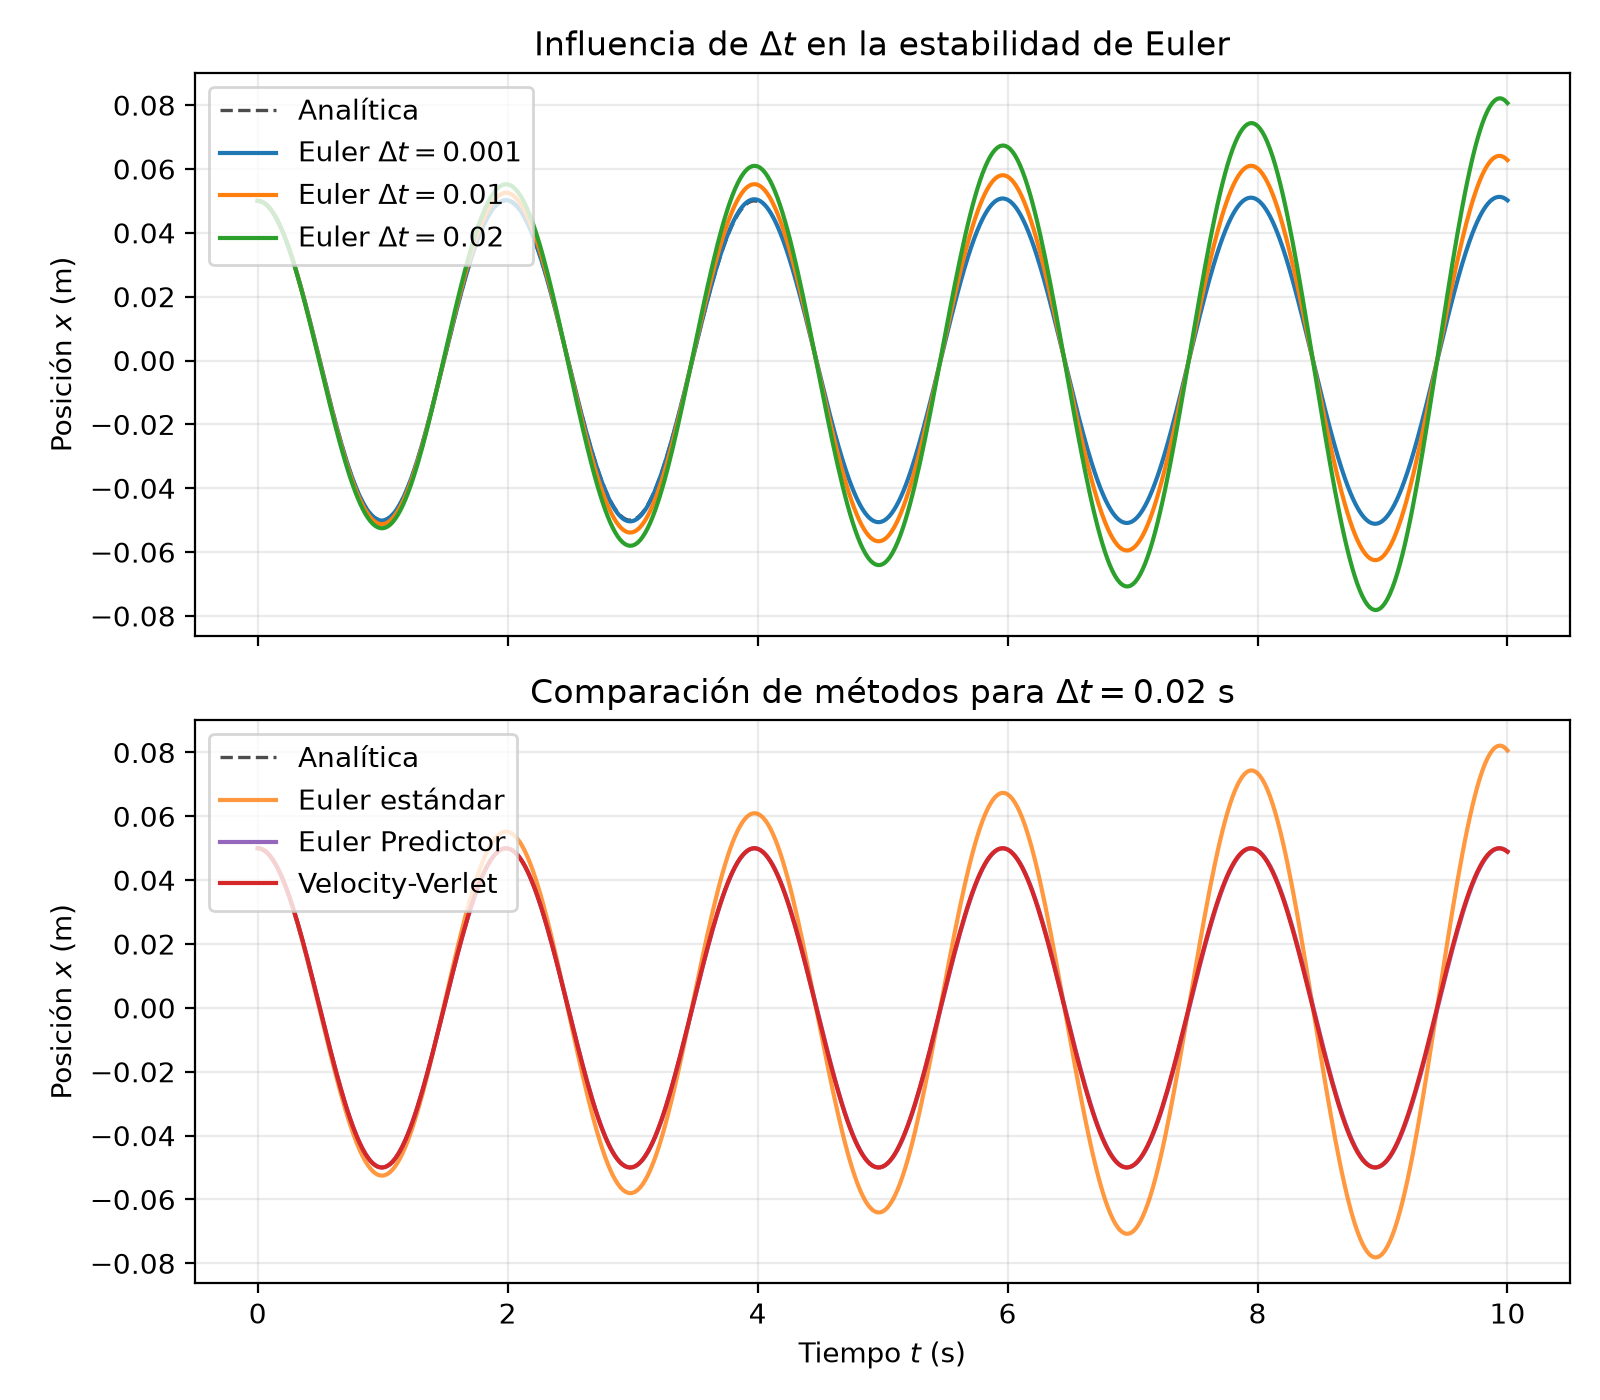
\includegraphics[width=0.78\linewidth]{../ex5/ex5_pos_plot.png}
  \caption{Oscillator position $x(t)$ over time. Top: Influence of $\Delta t \in \{0.001, 0.01, 0.02\}\text{ s}$ on the standard Euler method. Bottom: Comparison between standard Euler, Euler Predictor, and Velocity-Verlet for $\Delta t = 0.02\text{ s}$ against the analytical solution.}
  \label{fig:ex5_pos}
\end{figure}

The corresponding position errors $\vert{}x_{\text{num}}(t) - x_{\text{exact}}(t)\vert{}$ are shown on a logarithmic scale in Figure~\ref{fig:ex5_error}.

\begin{figure}[H]
  \centering
  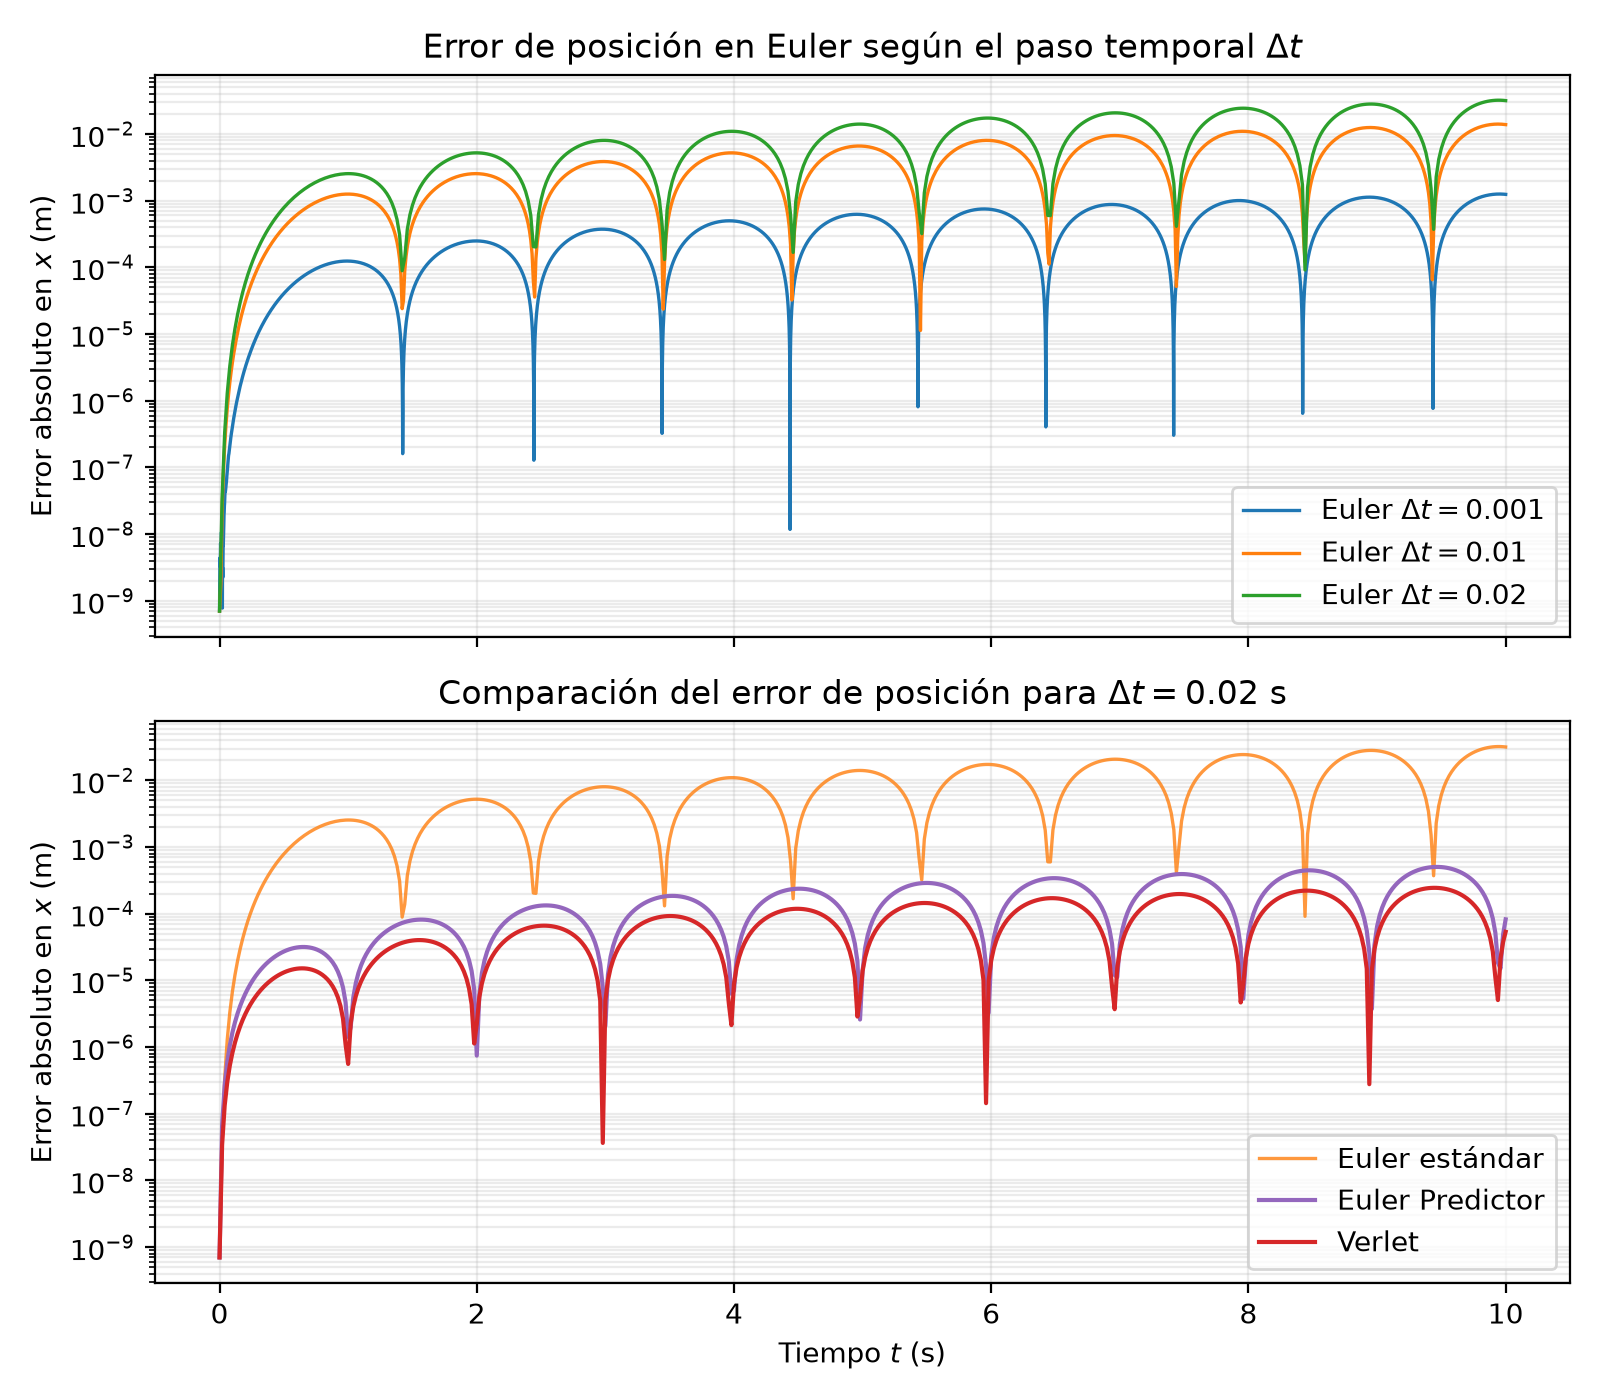
\includegraphics[width=0.78\linewidth]{../ex5/ex5_error_plot.png}
  \caption{Absolute error in position $\vert{}x_{\text{num}} - x_{\text{exact}}\vert{}$ (logarithmic scale). Top: Error in Euler's method as a function of $\Delta t$. Bottom: Numerical error comparison among the three algorithms for $\Delta t = 0.02\text{ s}$.}
  \label{fig:ex5_error}
\end{figure}

Figure~\ref{fig:ex5_energy} presents the individual energy balances (kinetic $E_k$, potential $E_p$, and total mechanical energy $E_{\text{tot}}$) for each algorithm at $\Delta t = 0.02\text{ s}$, comparing them with the exact reference $E_0 = 2.5\times 10^{-3}\text{ J}$.

\begin{figure}[H]
  \centering
  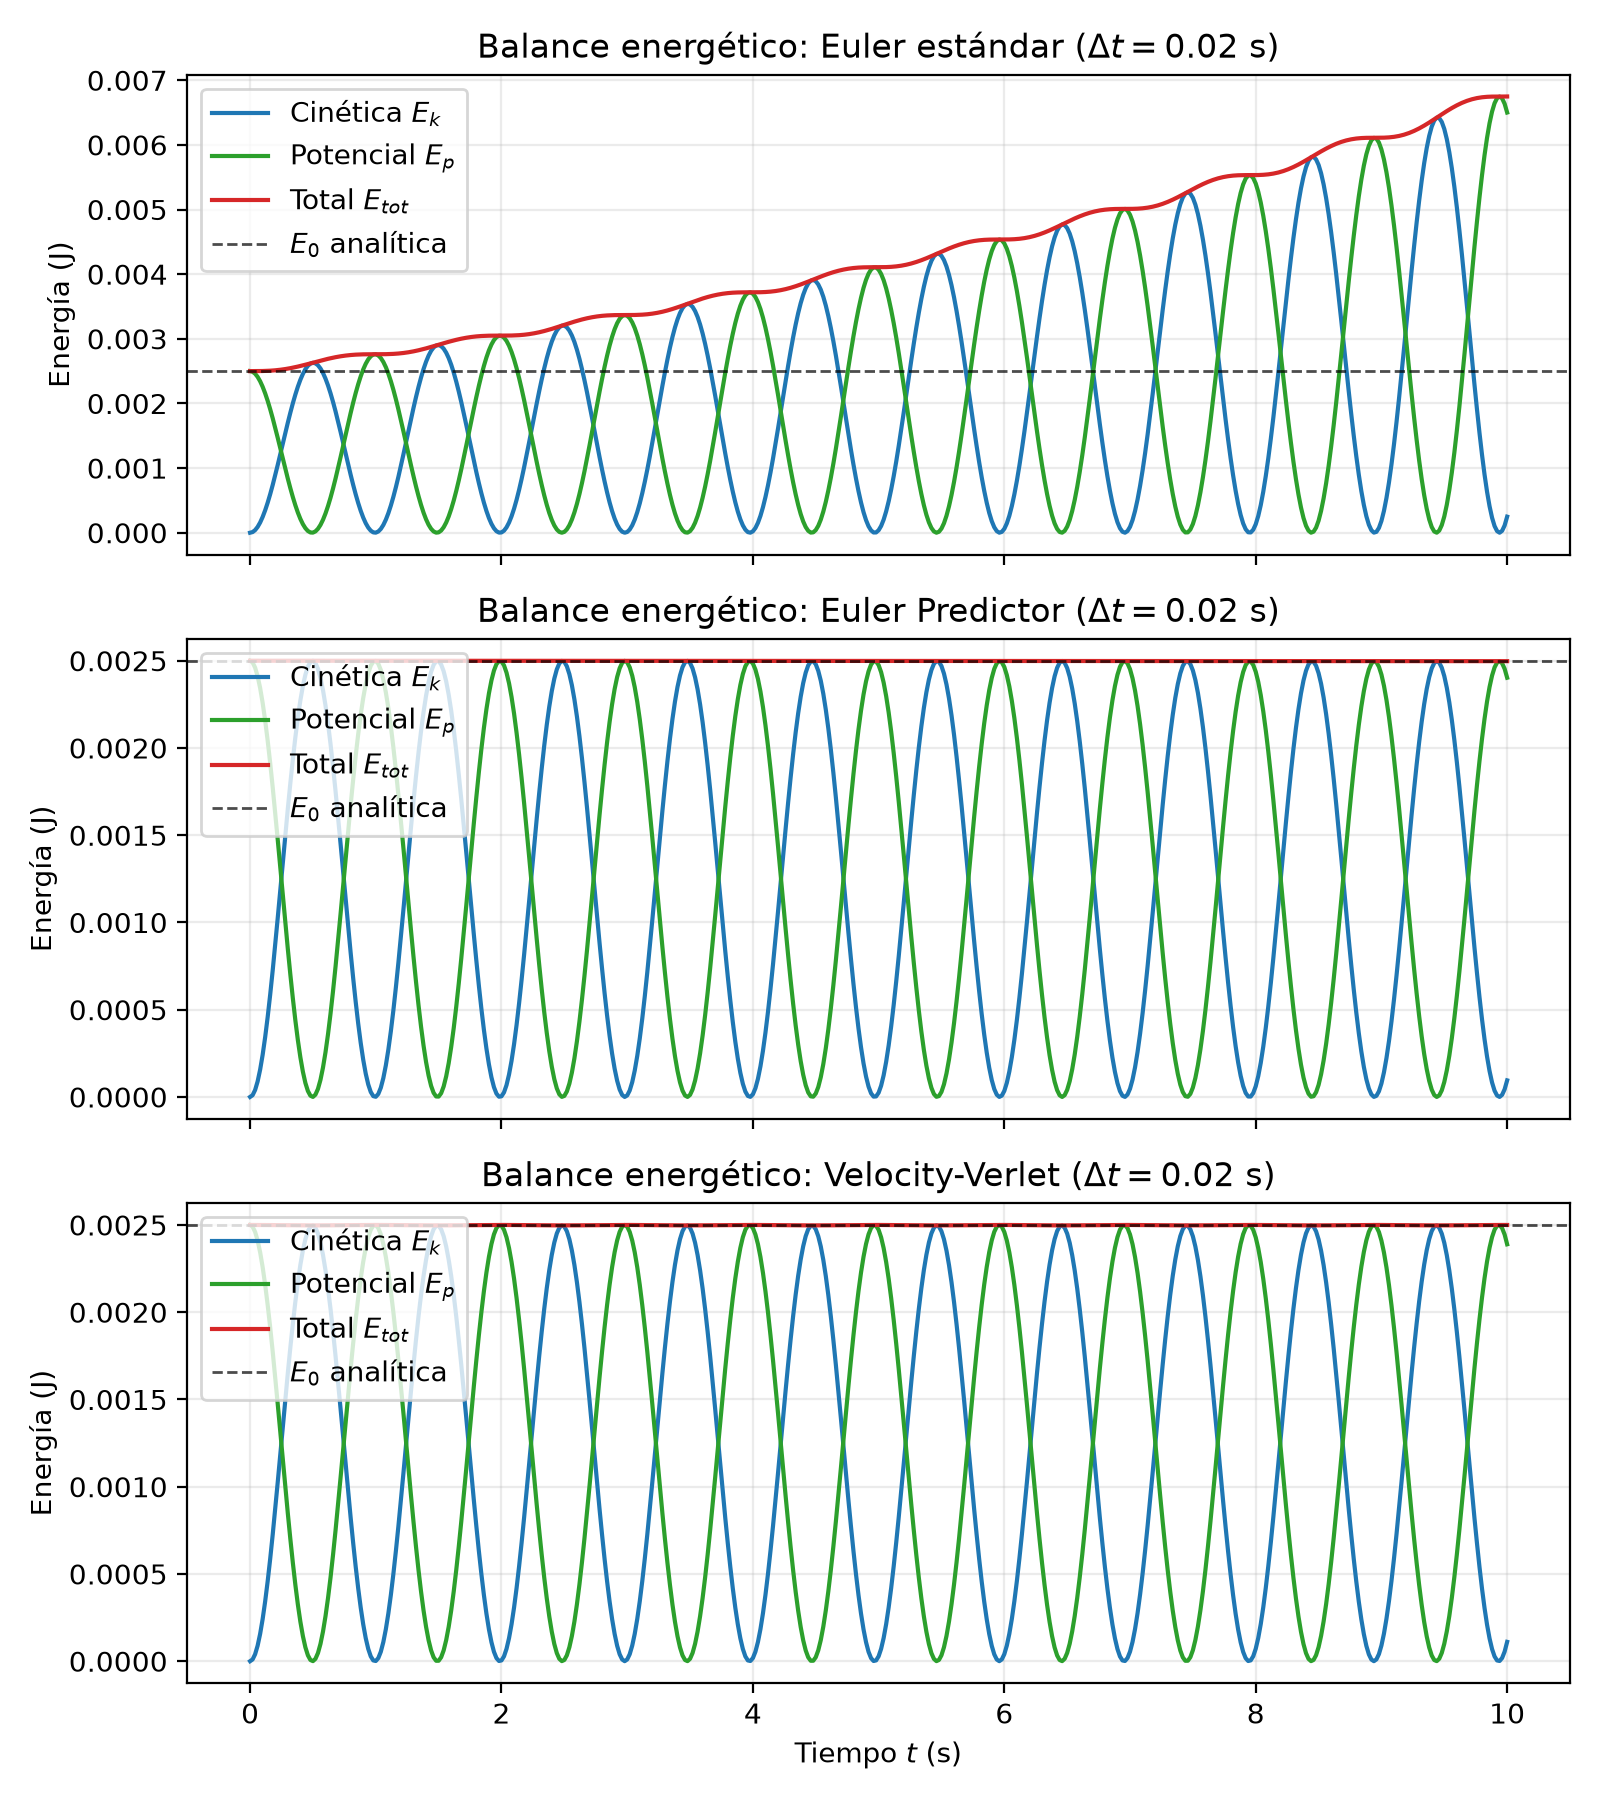
\includegraphics[width=0.78\linewidth]{../ex5/ex5_energy_plot.png}
  \caption{Kinetic, potential, and total energy evolution at $\Delta t = 0.02\text{ s}$. Top: Standard Euler. Middle: Euler Predictor. Bottom: Velocity-Verlet.}
  \label{fig:ex5_energy}
\end{figure}

A direct comparison of the total energy conservation $E_{\text{tot}}(t)$ among all three algorithms is displayed in Figure~\ref{fig:ex5_total_energy}. The absolute energy errors $\vert{}E_{\text{tot}}(t) - E_0\vert{}$ across step sizes and integration schemes are presented in Figure~\ref{fig:ex5_energy_error}.

\begin{figure}[H]
  \centering
  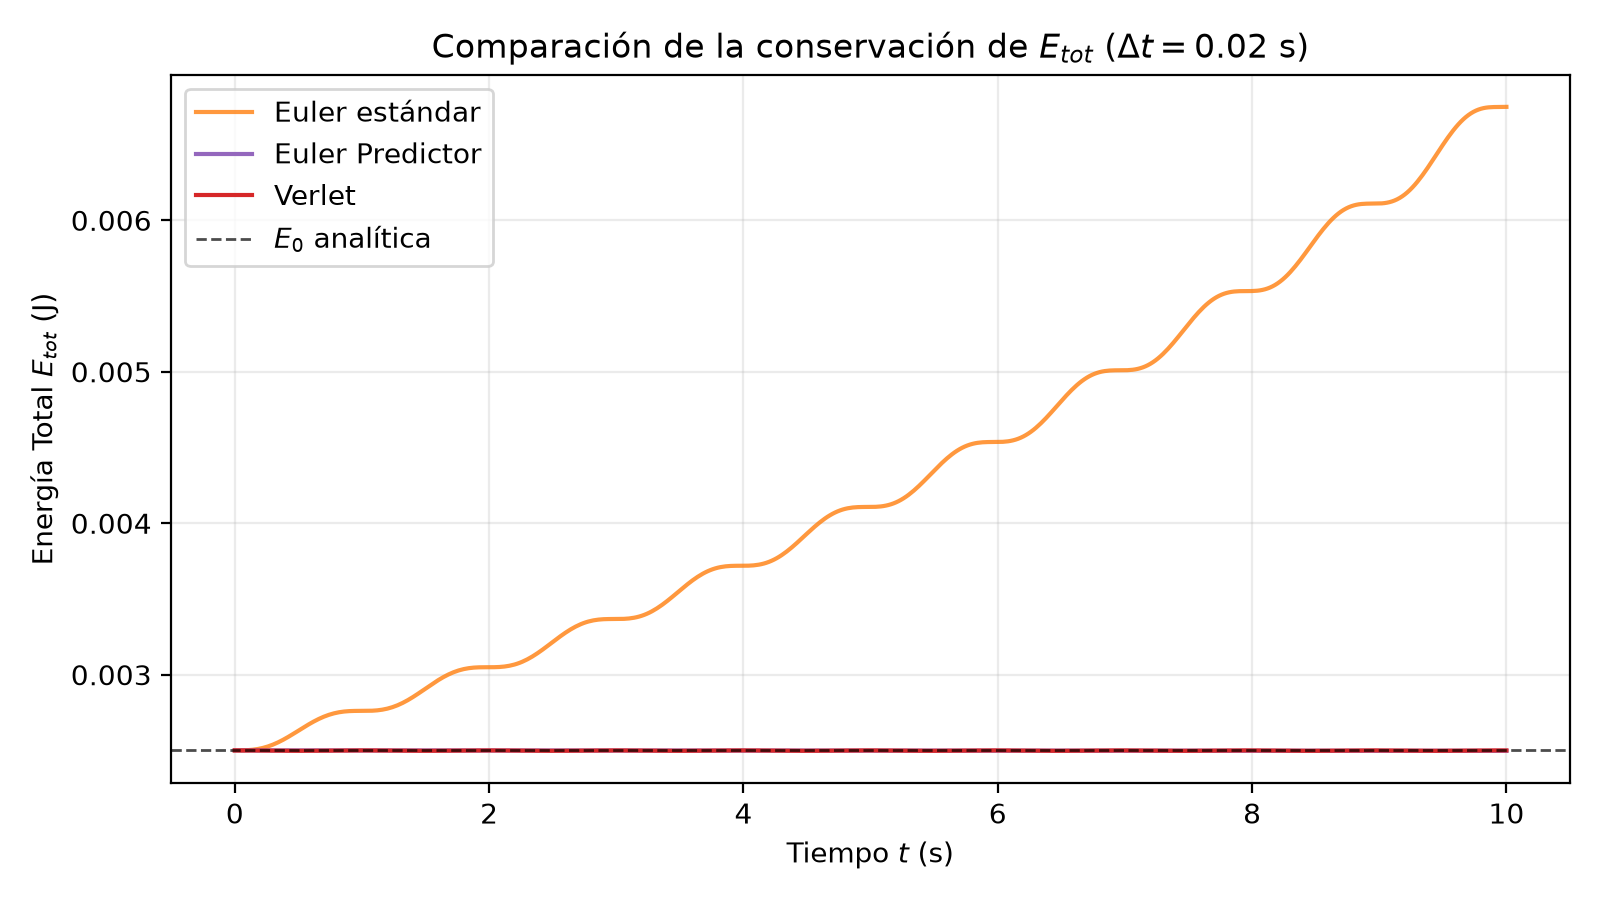
\includegraphics[width=0.78\linewidth]{../ex5/ex5_total_energy_plot.png}
  \caption{Comparison of total mechanical energy $E_{\text{tot}}(t)$ conservation between standard Euler, Euler Predictor, and Velocity-Verlet at $\Delta t = 0.02\text{ s}$.}
  \label{fig:ex5_total_energy}
\end{figure}

\begin{figure}[H]
  \centering
  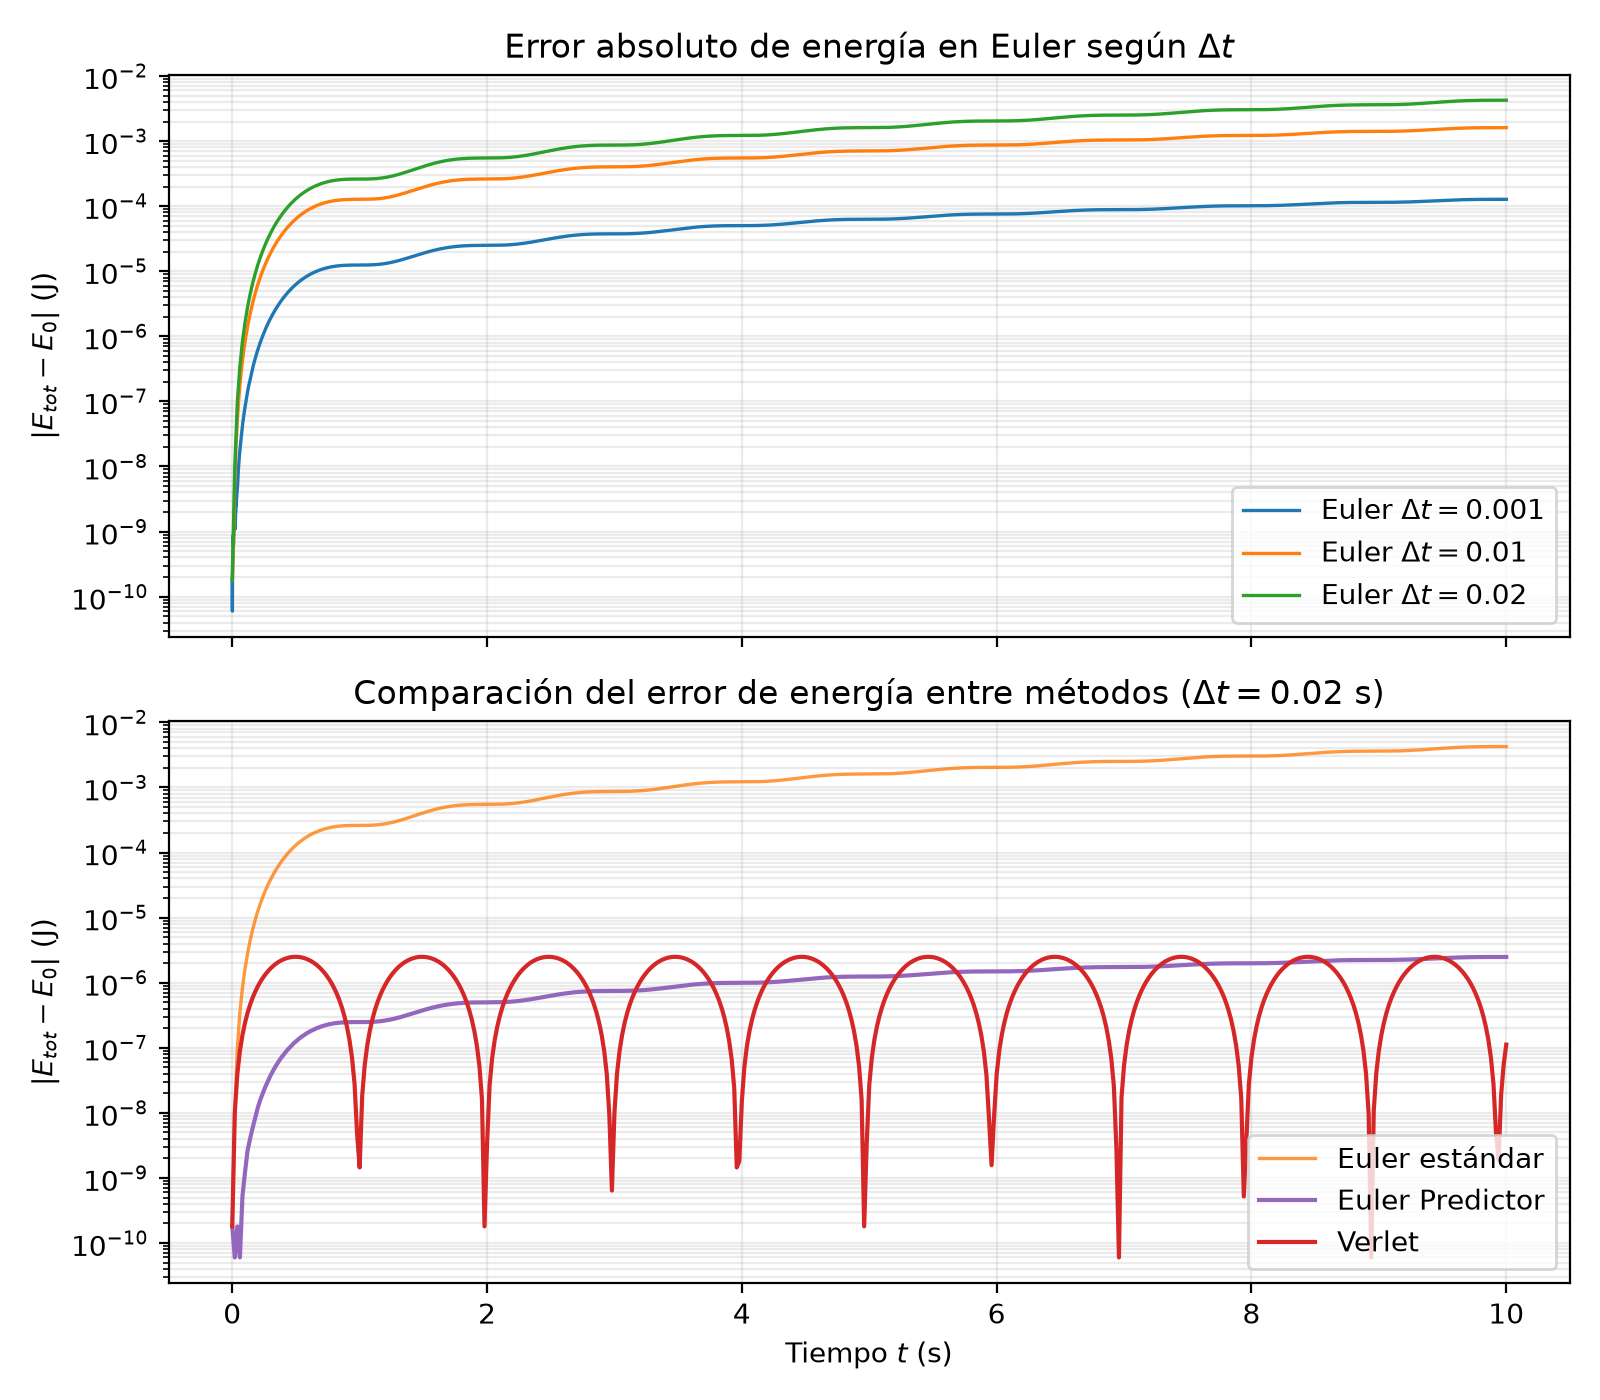
\includegraphics[width=0.78\linewidth]{../ex5/ex5_energy_error_plot.png}
  \caption{Absolute error in total energy $\vert{}E_{\text{tot}} - E_0\vert{}$ (logarithmic scale). Top: Effect of time step $\Delta t$ in Euler's method. Bottom: Comparison across the three methods for $\Delta t = 0.02\text{ s}$.}
  \label{fig:ex5_energy_error}
\end{figure}

\clearpage
\subsection{Discussion \& Notes}
\begin{itemize}
    \item \textbf{Influence of Time Step ($\Delta t$) on Euler's Method:} 
    As observed in both the trajectory and error curves, the explicit Euler method is highly sensitive to the choice of integration step size. For $\Delta t = 0.02\text{ s}$ and $\Delta t = 0.01\text{ s}$, the algorithm suffers from an intrinsic numerical instability that artificially amplifies the oscillation amplitude over time. Decreasing the step size to $\Delta t = 0.001\text{ s}$ significantly mitigates this growth and reduces the position error by over an order of magnitude ($\sim 10^{-3}\text{ m}$ compared to $\sim 3\times 10^{-2}\text{ m}$ for $\Delta t = 0.02\text{ s}$), though a gradual cumulative phase lag remains.

    \item \textbf{Performance Comparison Across Algorithms ($\Delta t = 0.02\text{ s}$):}
    Setting the step size to $\Delta t = 0.02\text{ s}$ clearly highlights the advantages of higher-order schemes over standard Euler:
    \begin{itemize}
        \item \emph{Standard Euler:} Demonstrates unbounded error growth reaching nearly $60\%$ of the initial amplitude by $t = 10\text{ s}$, making it unsuitable for long-term oscillatory dynamics.
        \item \emph{Euler Predictor-Corrector:} By averaging the predicted and current accelerations $\frac{1}{2}(a_n + a_{n+1}^{\text{pred}})$, the leading first-order truncation error terms cancel out, lowering the trajectory error down to $\sim 10^{-4}\text{ m}$.
        \item \emph{Velocity-Verlet:} Yields the closest agreement with the analytical trajectory $x(t) = x_0 \cos(\omega_0 t)$, keeping the numerical error bounded within $10^{-5}\text{ m}$ to $10^{-4}\text{ m}$ throughout the entire simulation interval.
    \end{itemize}

    \item \textbf{Mechanical Energy Conservation and Symplecticity:}
    The exact mechanical energy of the harmonic oscillator is constant:
    \begin{equation}
        E_0 = \frac{1}{2} k x_0^2 = \frac{1}{2} (2\text{ N/m}) (0.05\text{ m})^2 = 2.5 \times 10^{-3}\text{ J}
    \end{equation}
    Examining the energy balances illustrates the qualitative differences between the methods:
    \begin{itemize}
        \item In standard Euler, the phase shift between position and velocity causes a continuous, unphysical energy injection into the system. The total energy $E_{\text{tot}}$ undergoes an almost linear secular drift, nearly tripling to $E_{\text{tot}} \approx 6.7 \times 10^{-3}\text{ J}$ by $t = 10\text{ s}$.
        \item The Euler Predictor-Corrector scheme successfully bounds the total energy close to the nominal value, though without formal symplecticity it may exhibit slow drift over much longer integration times.
        \item Velocity-Verlet confirms its nature as a time-reversible, symplectic integrator. The kinetic and potential energies alternate symmetrically each quarter period, and total energy oscillates within tight bounds around $E_0$ without secular drift, making it the algorithm of choice for physical simulations and molecular dynamics.
    \end{itemize}
\end{itemize}
\end{document}